\documentclass[12pt,a4paper,reqno]{amsart}

% section handling
\usepackage{subfiles} 

% language
\usepackage[greek,english]{babel}
\usepackage[utf8]{inputenc}
\usepackage{alphabeta}

% change default names to greek
\addto\captionsenglish{
    \renewcommand{\contentsname}{Περιεχόμενα}
    \renewcommand{\refname}{Βιβλιογραφία}
    \renewcommand{\datename}{Ημερομηνία:}
    \renewcommand{\urladdrname}{Ιστοσελίδα}
}

% math 
\usepackage{amsmath,amsthm,amssymb,amscd}

% font
\usepackage[cal=euler]{mathalfa}
\usepackage{libertinus-type1}
% \usepackage{txfonts} % for upright greek letters
\usepackage{bm} % for bold symbols
\usepackage{bbm} % for the simply-looking bb symbols

% miscellaneous 
\usepackage{changepage} %for indenting environments
\usepackage{csquotes} % example: \textcquote{}
\usepackage{stmaryrd} % needed for \mapsfrom

% drawing
\usepackage{tikz,tikz-cd}
\usetikzlibrary{shapes.misc, patterns, matrix, calc, intersections,positioning}
\usepackage{graphics,graphicx}
\usepackage{float} % provides enhanced control and customization options for floating objects such as figures and tables

% colors
\usepackage{xcolor}
\definecolor{darkcandyapplered}{rgb}{0.64, 0.0, 0.0}
\definecolor{midnightblue}{rgb}{0.1, 0.1, 0.44}
\definecolor{mylightblue}{HTML}{336699}
\definecolor{burntorange}{rgb}{0.8, 0.33, 0.0}
\definecolor{iceberg}{rgb}{0.44, 0.65, 0.82}
\definecolor{applegreen}{rgb}{0.55, 0.71, 0.0}
\definecolor{canaryyellow}{rgb}{1.0, 0.94, 0.0}

% hrefs
\usepackage{hyperref}
\usepackage[noabbrev,capitalize]{cleveref}
\hypersetup{
    pdftoolbar=true,        
    pdfmenubar=true,        
    pdffitwindow=false,     
    pdfstartview={FitH},  % fits the width of the page to the window
    pdftitle={},
    pdfauthor={},
    pdfsubject={},
    pdfkeywords={},
    pdfnewwindow=true,  % links in new window
    colorlinks=true,  % false: boxed links; true: colored links
    linkcolor=darkcandyapplered,   % color of internal links
    citecolor=midnightblue,  % color of links to bibliography
    urlcolor=cyan,  % color of external links
    linktocpage=true  % changes the links from the section body to the page number
    }

% geometry
\textwidth=16cm 
\textheight=21cm 
\hoffset=-55pt 
\footskip=25pt

% thm envs
\theoremstyle{definition}
\newtheorem{remark}{Παρατήρηση}
\newtheorem*{example}{Παράδειγμα}
\newtheorem*{combInterlude}{Ιντερλούδιο Συνδυαστικής}

% math ops (you might need to change the path)
% In this macro I define all of my math operators

% fields
\newcommand{\NN}{\mathbbmss{N}} 
\newcommand{\ZZ}{\mathbbmss{Z}} 
\newcommand{\QQ}{\mathbbmss{Q}} 
\newcommand{\RR}{\mathbbmss{R}} 
\newcommand{\CC}{\mathbbmss{C}} 
\newcommand{\KK}{\mathbbmss{K}} 
\newcommand{\FF}{\mathbbmss{F}} 

% symmetric group
\newcommand{\fS}{\mathfrak{S}}  

% calligraphic 
\newcommand{\aA}{\mathcal{A}} 
\newcommand{\bB}{\mathcal{B}}
\newcommand{\cC}{\mathcal{C}}
\newcommand{\dD}{\mathcal{D}}
\newcommand{\eE}{\mathcal{E}}
\newcommand{\fF}{\mathcal{F}}
\newcommand{\hH}{\mathcal{H}}
\newcommand{\iI}{\mathcal{I}}
\newcommand{\lL}{\mathcal{L}}
\newcommand{\oO}{\mathcal{O}}
\newcommand{\pP}{\mathcal{P}}
\newcommand{\sS}{\mathcal{S}}
\newcommand{\mM}{\mathcal{M}}
\newcommand{\uU}{\mathcal{U}}

% bold
\newcommand{\bfa}{\mathbf{a}}
\newcommand{\bfe}{\mathbf{e}}
\newcommand{\bfF}{\pmb{F}}
\newcommand{\bfR}{\pmb{R}}
\newcommand{\bfv}{\mathbf{v}}
%\newcommand{\bfx}{\bm{x}}
%\newcommand{\bfx}{\mathbf{x}} 
\newcommand{\bfx}{\pmb{x}}
\newcommand{\bfX}{\pmb{X}}
\newcommand{\bfy}{\pmb{y}}
\newcommand{\bfz}{\pmb{z}}

% roman
\newcommand{\rmB}{\mathrm{B}}
\newcommand{\rmC}{\mathrm{C}}
\newcommand{\rmD}{\mathrm{D}} 
\newcommand{\rmI}{\mathrm{I}} 
\newcommand{\rmK}{\mathrm{K}}
\newcommand{\rmM}{\mathrm{M}}
\newcommand{\rmP}{\mathrm{P}}  
\newcommand{\rmQ}{\mathrm{Q}}  
\newcommand{\rmR}{\mathrm{R}}
\newcommand{\rmS}{\mathrm{S}}
\newcommand{\rmT}{\mathrm{T}}
\newcommand{\rmU}{\mathrm{U}}
\newcommand{\rmV}{\mathrm{V}}
\newcommand{\rmY}{\mathrm{Y}}
\newcommand{\rmZ}{\mathrm{Z}}

% greek letters
% I'm renewing some commands in order to appear in upright font
% If I want to change it later, I don't have to do it manually, I just change it from here.
% \newcommand{\uaa}{\alphaup}
% \renewcommand{\alpha}{\alphaup}
% \renewcommand{\beta}{\betaup}
% \renewcommand{\gamma}{\gammaup}
% \renewcommand{\delta}{\deltaup}
% \renewcommand{\epsilon}{\epsilonup}
% \newcommand{\ee}{\epsilon}
% \renewcommand{\varepsilon}{\varepsilonup}
% \renewcommand{\theta}{\thetaup}
% \renewcommand{\lambda}{\lambdaup}
% \newcommand{\ull}{\lambda}
% \renewcommand{\mu}{\muup}
% \renewcommand{\nu}{\nuup}
% \renewcommand{\pi}{\piup}
% \renewcommand{\rho}{\rhoup}
% \renewcommand{\varrho}{\varrhoup}
% \renewcommand{\sigma}{\sigmaup}
% \renewcommand{\tau}{\tauup} 
% \renewcommand{\phi}{\phiup}
% \renewcommand{\chi}{\chiup}
% \renewcommand{\psi}{\psiup}
% \renewcommand{\omega}{\omegaup}

% arrows and symbols 
\renewcommand{\to}{\rightarrow}
\newcommand{\toto}{\longrightarrow}
\newcommand{\mapstoto}{\longmapsto}
\newcommand{\then}{\Rightarrow}
\newcommand{\IFF}{\Leftrightarrow}
\newcommand{\tl}{\tilde}
\newcommand{\wtl}{\widetilde}
\newcommand{\ol}{\overline}
\newcommand{\ul}{\underline}
\newcommand{\oldemptyset}{\emptyset}
\renewcommand{\emptyset}{\varnothing}
\DeclareMathSymbol{\Arg}{\mathbin}{AMSa}{"39} % for arguments 
\newcommand{\onto}{\ensuremath{\twoheadrightarrow}}

% absolute value symbol
\usepackage{mathtools} 
\DeclarePairedDelimiter\abs{\lvert}{\rvert}%
\DeclarePairedDelimiter\norm{\lVert}{\rVert}%
\makeatletter
\let\oldabs\abs
\def\abs{\@ifstar{\oldabs}{\oldabs*}}

% tensor symbol
\newcommand{\tensor}[1]{%
  \mathbin{\mathop{\otimes}\limits_{#1}}%
}

% permutation cycle notation
\ExplSyntaxOn
\NewDocumentCommand{\cycle}{ O{\;} m }
 {
  (
  \alec_cycle:nn { #1 } { #2 }
  )
 }

\seq_new:N \l_alec_cycle_seq
\cs_new_protected:Npn \alec_cycle:nn #1 #2
 {
  \seq_set_split:Nnn \l_alec_cycle_seq { , } { #2 }
  \seq_use:Nn \l_alec_cycle_seq { #1 }
 }
\ExplSyntaxOff

% setminus symbol
\newcommand{\mysetminusD}{\hbox{\tikz{\draw[line width=0.6pt,line cap=round] (3pt,0) -- (0,6pt);}}}
\newcommand{\mysetminusT}{\mysetminusD}
\newcommand{\mysetminusS}{\hbox{\tikz{\draw[line width=0.45pt,line cap=round] (2pt,0) -- (0,4pt);}}}
\newcommand{\mysetminusSS}{\hbox{\tikz{\draw[line width=0.4pt,line cap=round] (1.5pt,0) -- (0,3pt);}}}
\newcommand{\sm}{\mathbin{\mathchoice{\mysetminusD}{\mysetminusT}{\mysetminusS}{\mysetminusSS}}}

% custom math operators
\newcommand{\Des}{\mathrm{Des}} 
\newcommand{\des}{\mathrm{des}} 
\newcommand{\Asc}{\mathrm{Asc}}
\newcommand{\asc}{\mathrm{asc}} 
\newcommand{\inv}{\mathrm{inv}}
\newcommand{\Inv}{\mathrm{Inv}}
\newcommand{\maj}{\mathrm{maj}} 
\newcommand{\comaj}{\mathrm{comaj}} 
\newcommand{\fix}{\mathrm{fix}} 
\newcommand{\Sym}{\mathrm{Sym}} 
\newcommand{\QSym}{\mathrm{QSym}}
\newcommand{\FQSym}{\mathrm{FQSym}} 
\newcommand{\End}{\mathrm{End}} 
\newcommand{\Rad}{\mathrm{Rad}} 
\newcommand{\rmMat}{\mathrm{Mat}} 
\newcommand{\rmdim}{\mathrm{dim}} 
\newcommand{\rmTop}{\mathrm{Top}} 
\newcommand{\rmCF}{\mathrm{CF}} 
\newcommand{\rmId}{\mathrm{Id}}
\newcommand{\rmid}{\mathrm{id}}
\newcommand{\rmtw}{\mathrm{tw}}
\newcommand{\trace}{\mathrm{tr}}
\newcommand{\Irr}{\mathrm{Irr}}
\newcommand{\Ind}{\mathrm{Ind}} % induction
\newcommand{\Res}{\mathrm{Res}} % restriction
\newcommand{\triv}{\mathrm{triv}} % trivial rep
\newcommand{\rmdef}{\mathrm{def}} % defining rep
\newcommand{\dom}{\triangleleft}
\newcommand{\domeq}{\trianglelefteq}
\newcommand{\lex}{\mathrm{lex}}
\newcommand{\sign}{\mathrm{sign}}
\newcommand{\SYT}{\mathrm{SYT}}
\renewcommand{\Im}{\mathrm{Im}}
\newcommand{\Ker}{\mathrm{Ker}}
\newcommand{\GL}{\mathrm{GL}}
\newcommand{\FL}{\mathrm{FL}}
\newcommand{\Span}{\mathrm{span}}
\newcommand{\pos}{\mathrm{pos}}
\newcommand{\Comp}{\mathrm{Comp}}
\newcommand{\Set}{\mathrm{Set}}
\newcommand{\std}{\mathrm{std}}
\newcommand{\cont}{\mathrm{cont}} %content of a SSYT
\newcommand{\SSYT}{\mathrm{SSYT}}
\newcommand{\rmz}{\mathrm{z}}
\newcommand{\ct}{\mathrm{ct}} % cycle type
\newcommand{\ch}{\mathrm{ch}} % Frobenius characteristic map
\newcommand{\height}{\mathrm{ht}}
\newcommand{\FPS}{\CC[\![\bfx]\!]} % formal power series
\newcommand{\FPSS}{\CC[\![\bfx,\bfy]\!]}
\newcommand{\reg}{\mathrm{reg}}
\newcommand{\hook}{\mathrm{h}}
\newcommand{\weight}{\mathrm{wt}}
\newcommand{\co}{\mathrm{co}}
\newcommand{\ps}{\mathrm{ps}}
\newcommand{\rmsum}{\mathrm{sum}}
\newcommand{\NSym}{\mathrm{NSym}}
\newcommand{\Hom}{\mathrm{Hom}}
\newcommand{\proj}{\mathrm{proj}}
\newcommand{\stat}{\mathrm{stat}}

% miscellaneous commands
\newcommand{\defn}[1]{{\color{mylightblue}{#1}}}
\newcommand{\toDo}{{\bf\color{red} TODO}}
\newcommand{\toCite}{{\bf\color{green} CITE}}

% 
\newenvironment{nouppercase}{%
  \let\uppercase\relax%
  \renewcommand{\uppercasenonmath}[1]{}}{}

\newcommand{\one}{\textcolor{iceberg}{1}}
\newcommand{\two}{\textcolor{burntorange}{2}}
\newcommand{\three}{\textcolor{applegreen}{3}}
\newcommand{\four}{\textcolor{canaryyellow}{4}}

% titlepage
\title{Θ2.04: Θεωρία Αναπαραστάσεων και Συνδυαστική}
\author[Β.~Δ. Μουστακας]{Βασίλης Διονύσης Μουστάκας \\ Πανεπιστήμιο Κρήτης}
\date{8 Οκτωβρίου 2025}
% \urladdr{\href{https://sites.google.com/view/vasmous}{https://sites.google.com/view/vasmous}}

\begin{document}

\begingroup
\def\uppercasenonmath#1{} % this disables uppercase title
\let\MakeUppercase\relax % this disables uppercase authors
\maketitle
\endgroup

% \setcounter{section}{}
\thispagestyle{empty}

\begin{center}
    \textbf{Παραδείγματα ομάδων, δράσεων και αναπαραστάσεων
}
\end{center}

Έστω $\rmD_{2n}$ η ομάδα συμμετρίας ενός κανονικού $n$-γώνου, η οποία ονομάζεται \defn{διεδρική ομάδα}, και έχει τάξη $2n$. Για $n=3$ και $n=4$ έχουμε τις εξής συμμετρίες:
\[
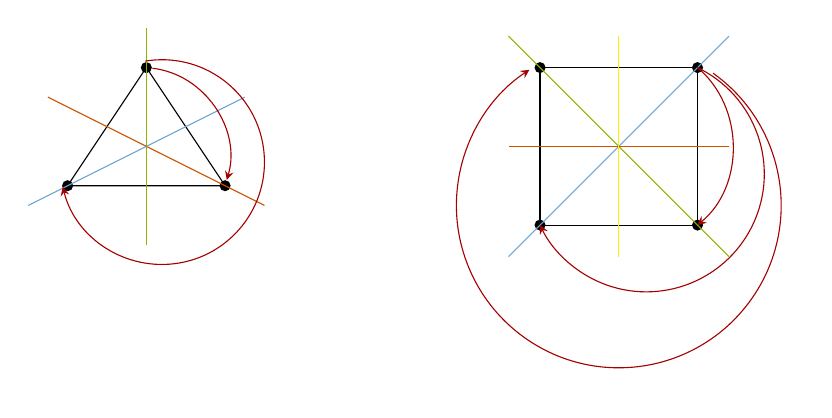
\begin{tikzpicture}[>=stealth]
    \begin{scope}[shift={(0,-.5)}]
        \tikzstyle{point}=[circle,fill,inner sep=0pt, minimum width=4pt, minimum height=4pt]

        % Triangle vertices
        \node (e3)[point] at (1,1.5) {};
        \node (e1)[point] at (2,0) {};
        \node (e2)[point] at (0,0) {};

        % Barycenter
        \coordinate (bary) at (1,0.5) {}; 

        % Draw the triangle
        \draw (e1.center) -- (e2.center) -- (e3.center) -- cycle;

        % Compute extended axis endpoints
        \coordinate (e1_ext) at ($(bary) !1.5! (e1)$);
        \coordinate (e2_ext) at ($(bary) !1.5! (e2)$);
        \coordinate (e3_ext) at ($(bary) !1.5! (e3)$);

        % Draw coordinate axes
        \draw[burntorange] (bary.center) -- (e1_ext);
        \draw[iceberg] (bary.center) -- (e2_ext);
        \draw[applegreen] (bary.center) -- (e3_ext);

        % Make the e2 axis red and extend it beyond the midpoint of e1-e3
        \coordinate (mid_e1_e2) at ($(e1)!0.5!(e2)$); % Midpoint of e1 and e2
        \coordinate (mid_e1_e3) at ($(e1)!0.5!(e3)$); % Midpoint of e1 and e3
        \coordinate (mid_e2_e3) at ($(e2)!0.5!(e3)$); % Midpoint of e2 and e3
        \coordinate (e1_extended) at ($(e1)!1.5!(mid_e2_e3)$); % Extend e1 axis beyond midpoint
        \coordinate (e2_extended) at ($(e2)!1.5!(mid_e1_e3)$); % Extend e2 axis beyond midpoint
        \coordinate (e3_extended) at ($(e3)!1.5!(mid_e1_e2)$); % Extend e3 axis beyond midpoint
        \draw[applegreen] (bary.center) -- (e3_extended); % Red e3 axis extended
        \draw[iceberg] (bary.center) -- (e2_extended); % Red e2 axis extended
        \draw[burntorange] (bary.center) -- (e1_extended); % Red e1 axis extended

        % Curved arrows showing clockwise direction around the triangle
        \draw[darkcandyapplered, ->, bend left=50] (e3) to (e1);

        \coordinate (center) at (1.2,0.3);
        \def\radius{1.3}

        % Draw the full circle for reference
        % \draw[gray,dashed] (center) circle[radius=\radius];

        % Compute polar angles of e3 and e2 relative to the center
        \pgfmathanglebetweenpoints{\pgfpointanchor{center}{center}}{\pgfpointanchor{e3}{center}}
        \let\startangle\pgfmathresult
        \pgfmathanglebetweenpoints{\pgfpointanchor{center}{center}}{\pgfpointanchor{e2}{center}}
        \let\endangle\pgfmathresult

        % Draw the COMPLEMENTARY arc (the other part of the same circle)
        % The key is to add or subtract 360 degrees to go the long way around
        \draw[darkcandyapplered,->]
        (center) ++(\startangle:\radius)
        arc[start angle=\startangle, end angle=\endangle-360, radius=\radius];
    \end{scope}

    \begin{scope}[shift={(7,0)}]
        \tikzstyle{point}=[circle,fill,inner sep=0pt, minimum width=4pt, minimum height=4pt]
          % Square vertices
        \coordinate (v1) at (1,1);    % upper right
        \coordinate (v2) at (1,-1);   % lower right
        \coordinate (v3) at (-1,-1);  % lower left
        \coordinate (v4) at (-1,1);   % upper left

        % center (barycenter)
        \coordinate (O) at (0,0);

        % midpoints of edges (medians direction)
        \coordinate (m12) at ($(v1)!0.5!(v2)$); % (1,0)
        \coordinate (m23) at ($(v2)!0.5!(v3)$); % (0,-1)
        \coordinate (m34) at ($(v3)!0.5!(v4)$); % (-1,0)
        \coordinate (m41) at ($(v4)!0.5!(v1)$); % (0,1)

        % Draw square
        \draw (v1) -- (v2) -- (v3) -- (v4) -- cycle;

        % Draw vertices as filled points and label
        \node[point] at (v1) {};
        \node[point] at (v2) {};
        \node[point] at (v3) {};
        \node[point] at (v4) {};

        % Symmetry lines (extended past the square)
        % Diagonal v1<->v3
        \draw[iceberg]
            ($(O)!1.4!(v1)$) -- ($(O)!-1.4!(v1)$);

        % Diagonal v2<->v4
        \draw[applegreen]
            ($(O)!1.4!(v2)$) -- ($(O)!-1.4!(v2)$);

        % Median horizontal (through midpoints m12 and m34)
        \draw[burntorange]
            ($(O)!1.4!(m12)$) -- ($(O)!-1.4!(m12)$);

        % Median vertical (through midpoints m23 and m41)
        \draw[canaryyellow]
            ($(O)!1.4!(m23)$) -- ($(O)!-1.4!(m23)$);

        \draw[darkcandyapplered, ->, bend left=50] (v1) to (v2);
        
        
        % --- Circle 1: passes exactly through v1 and v3  ---
        \coordinate (C13) at (0.35,-0.35);

        \path let \p1=(C13), \p2=(v1), \p3=(v3) in
        \pgfextra{
            \pgfmathsetmacro{\radiusAtemp}{veclen(\x1-\x2,\y1-\y2)}
            \pgfmathsetmacro{\startAtemp}{atan2(\y2-\y1,\x2-\x1)}
            \pgfmathsetmacro{\endAtemp}{atan2(\y3-\y1,\x3-\x1)}
            \pgfmathsetmacro{\deltaAtemp}{mod(360-(\endAtemp-\startAtemp),360)}
            \xdef\radiusA{\radiusAtemp}
            \xdef\startA{\startAtemp}
            \xdef\endA{\endAtemp}
            \xdef\deltaA{\deltaAtemp}
        };

        \draw[darkcandyapplered,->]
        (C13) ++(\startA:\radiusA pt)
        arc[start angle=\startA, delta angle=-\deltaA, radius=\radiusA pt];


        % --- Large arc through v1, v4:
        \coordinate (C14) at (0,-0.75);
        \draw[darkcandyapplered,->]
        (C14) ++(54.4623:2.0625cm)
        arc[start angle=54.4623, delta angle=-291.0754, radius=2.0625cm];
    \end{scope}
\end{tikzpicture}
\]

Αν συμβολίσουμε με $r$ την στροφή κατά την φορά του ρολογιού κατά $2\pi/n$, και $s$ την ανάκλαση ως προς την ευθεία που περνάει από την βαρύκεντρο και μια κορυφή του κανονικού $n$-γώνου, την οποία έχουμε σταθεροποιήσει\footnote{Αν ο $n$ είναι περιττός, τότε αυτή περνάει από το μέσο της απέναντι πλευράς, ενώ αν ο $n$ είναι άρτιος, τότε περνάει από την απέναντι κορυφή (γιατί;).}, τότε παρατηρούμε ότι 
\begin{itemize}
    \item τα $\epsilon, r, r^2, \dots, r^{n-1}$ είναι διαφορετικά
    \item $sr^i \neq sr^j$, για κάθε $1 \le i \neq j \le n-1$ 
    \item $r^n = s^2 = \epsilon$
    \item $rsr = s$.
\end{itemize}

Για παράδειγμα, για $n=4$ οι συμμετρίες $sr, sr^2$ και $sr^3$ σχηματικά δίνονται από:
\[
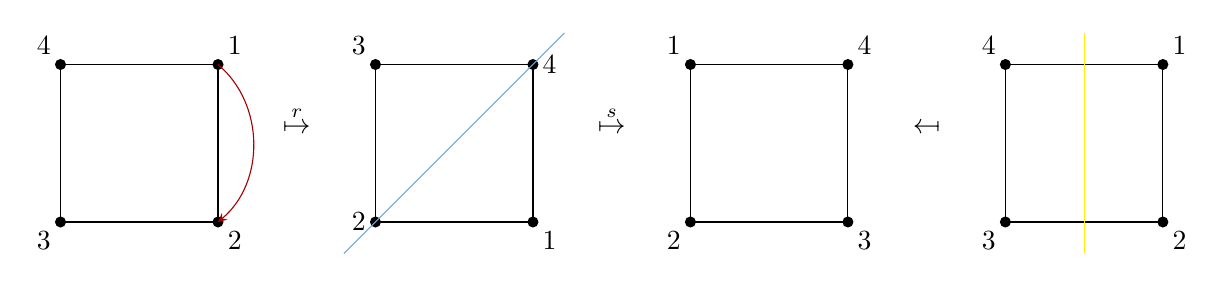
\begin{tikzpicture}[>=stealth]
    \tikzstyle{point}=[circle,fill,inner sep=0pt, minimum width=4pt, minimum height=4pt]
    \begin{scope}[shift={(0,0)}]
        % Square vertices
        \coordinate[label=above right:{1}] (v1) at (1,1);    % upper right
        \coordinate[label=below right:{2}] (v2) at (1,-1);   % lower right
        \coordinate[label=below left:{3}] (v3) at (-1,-1);  % lower left
        \coordinate[label=above left:{4}] (v4) at (-1,1);   % upper lef
        \node[point] at (v1) {};
        \node[point] at (v2) {};
        \node[point] at (v3) {};
        \node[point] at (v4) {};
        % center (barycenter)
        \coordinate (O) at (0,0);
        % midpoints of edges (medians direction)
        \coordinate (m12) at ($(v1)!0.5!(v2)$); % (1,0)
        \coordinate (m23) at ($(v2)!0.5!(v3)$); % (0,-1)
        \coordinate (m34) at ($(v3)!0.5!(v4)$); % (-1,0)
        \coordinate (m41) at ($(v4)!0.5!(v1)$); % (0,1)
        % Draw square
        \draw (v1) -- (v2) -- (v3) -- (v4) -- cycle;
        % rot v1->v2
        \draw[darkcandyapplered, ->, bend left=50] (v1) to (v2);
    \end{scope}

    \coordinate[label={$\stackrel{r}{\mapsto}$}] (x) at (2,0);

    \begin{scope}[shift={(4,0)}]
        % Square vertices
        \coordinate[label=right:{4}] (v1) at (1,1);    % upper right
        \coordinate[label=below right:{1}] (v2) at (1,-1);   % lower right
        \coordinate[label=left:{2}] (v3) at (-1,-1);  % lower left
        \coordinate[label=above left:{3}] (v4) at (-1,1);   % upper lef
        \node[point] at (v1) {};
        \node[point] at (v2) {};
        \node[point] at (v3) {};
        \node[point] at (v4) {};
        % center (barycenter)
        \coordinate (O) at (0,0);
        % midpoints of edges (medians direction)
        \coordinate (m12) at ($(v1)!0.5!(v2)$); % (1,0)
        \coordinate (m23) at ($(v2)!0.5!(v3)$); % (0,-1)
        \coordinate (m34) at ($(v3)!0.5!(v4)$); % (-1,0)
        \coordinate (m41) at ($(v4)!0.5!(v1)$); % (0,1)
        % Draw square
        \draw (v1) -- (v2) -- (v3) -- (v4) -- cycle;
        % Diagonal v1<->v3
        \draw[iceberg] ($(O)!1.4!(v1)$) -- ($(O)!-1.4!(v1)$);
    \end{scope}

    \coordinate[label={$\stackrel{s}{\mapsto}$}] (xx) at (6,0);

    \begin{scope}[shift={(8,0)}]
        % Square vertices
        \coordinate[label=above right:{4}] (v1) at (1,1);    % upper right
        \coordinate[label=below right:{3}] (v2) at (1,-1);   % lower right
        \coordinate[label=below left:{2}] (v3) at (-1,-1);  % lower left
        \coordinate[label=above left:{1}] (v4) at (-1,1);   % upper lef
        \node[point] at (v1) {};
        \node[point] at (v2) {};
        \node[point] at (v3) {};
        \node[point] at (v4) {};
        % center (barycenter)
        \coordinate (O) at (0,0);
        % midpoints of edges (medians direction)
        \coordinate (m12) at ($(v1)!0.5!(v2)$); % (1,0)
        \coordinate (m23) at ($(v2)!0.5!(v3)$); % (0,-1)
        \coordinate (m34) at ($(v3)!0.5!(v4)$); % (-1,0)
        \coordinate (m41) at ($(v4)!0.5!(v1)$); % (0,1)
        % Draw square
        \draw (v1) -- (v2) -- (v3) -- (v4) -- cycle;
    \end{scope}

    \coordinate[label={$\mapsfrom$}] (xxx) at (10,0);

    \begin{scope}[shift={(12,0)}]
        % Square vertices
        \coordinate[label=above right:{1}] (v1) at (1,1);    % upper right
        \coordinate[label=below right:{2}] (v2) at (1,-1);   % lower right
        \coordinate[label=below left:{3}] (v3) at (-1,-1);  % lower left
        \coordinate[label=above left:{4}] (v4) at (-1,1);   % upper lef
        % Draw vertices as filled points and label
        \node[point] at (v1) {};
        \node[point] at (v2) {};
        \node[point] at (v3) {};
        \node[point] at (v4) {};
        % center (barycenter)
        \coordinate (O) at (0,0);
        % midpoints of edges (medians direction)
        \coordinate (m12) at ($(v1)!0.5!(v2)$); % (1,0)
        \coordinate (m23) at ($(v2)!0.5!(v3)$); % (0,-1)
        \coordinate (m34) at ($(v3)!0.5!(v4)$); % (-1,0)
        \coordinate (m41) at ($(v4)!0.5!(v1)$); % (0,1)
        % Draw square
        \draw (v1) -- (v2) -- (v3) -- (v4) -- cycle;
        % Median vertical (through midpoints m23 and m41)
        \draw[canaryyellow]
            ($(O)!1.4!(m23)$) -- ($(O)!-1.4!(m23)$);
    \end{scope}
\end{tikzpicture}
\]

\[
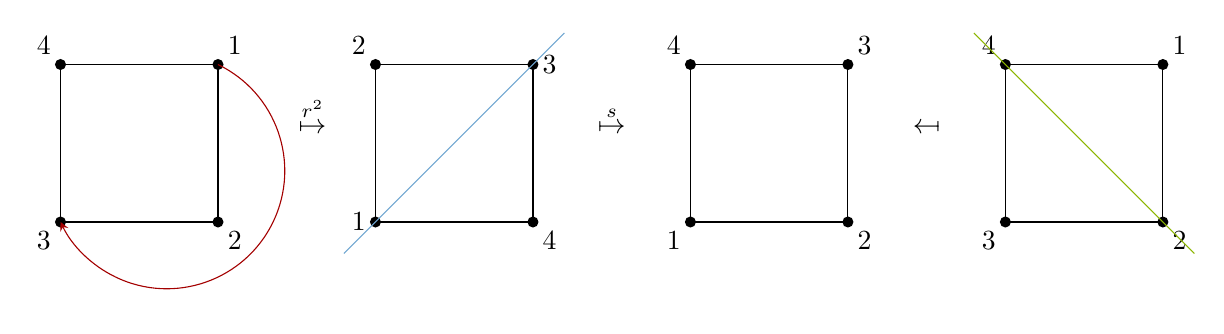
\begin{tikzpicture}[>=stealth]
    \tikzstyle{point}=[circle,fill,inner sep=0pt, minimum width=4pt, minimum height=4pt]
    \begin{scope}[shift={(0,0)}]
        % Square vertices
        \coordinate[label=above right:{1}] (v1) at (1,1);    % upper right
        \coordinate[label=below right:{2}] (v2) at (1,-1);   % lower right
        \coordinate[label=below left:{3}] (v3) at (-1,-1);  % lower left
        \coordinate[label=above left:{4}] (v4) at (-1,1);   % upper lef
        \node[point] at (v1) {};
        \node[point] at (v2) {};
        \node[point] at (v3) {};
        \node[point] at (v4) {};
        % center (barycenter)
        \coordinate (O) at (0,0);
        % midpoints of edges (medians direction)
        \coordinate (m12) at ($(v1)!0.5!(v2)$); % (1,0)
        \coordinate (m23) at ($(v2)!0.5!(v3)$); % (0,-1)
        \coordinate (m34) at ($(v3)!0.5!(v4)$); % (-1,0)
        \coordinate (m41) at ($(v4)!0.5!(v1)$); % (0,1)
        % Draw square
        \draw (v1) -- (v2) -- (v3) -- (v4) -- cycle;
        % rot v1->v3
        % --- Circle 1: passes exactly through v1 and v3  ---
        \coordinate (C13) at (0.35,-0.35);

        \path let \p1=(C13), \p2=(v1), \p3=(v3) in
        \pgfextra{
            \pgfmathsetmacro{\radiusAtemp}{veclen(\x1-\x2,\y1-\y2)}
            \pgfmathsetmacro{\startAtemp}{atan2(\y2-\y1,\x2-\x1)}
            \pgfmathsetmacro{\endAtemp}{atan2(\y3-\y1,\x3-\x1)}
            \pgfmathsetmacro{\deltaAtemp}{mod(360-(\endAtemp-\startAtemp),360)}
            \xdef\radiusA{\radiusAtemp}
            \xdef\startA{\startAtemp}
            \xdef\endA{\endAtemp}
            \xdef\deltaA{\deltaAtemp}
        };

        \draw[darkcandyapplered,->]
        (C13) ++(\startA:\radiusA pt)
        arc[start angle=\startA, delta angle=-\deltaA, radius=\radiusA pt];
    \end{scope}

    \coordinate[label={$\stackrel{r^2}{\mapsto}$}] (x) at (2.2,0);

    \begin{scope}[shift={(4,0)}]
        % Square vertices
        \coordinate[label=right:{3}] (v1) at (1,1);    % upper right
        \coordinate[label=below right:{4}] (v2) at (1,-1);   % lower right
        \coordinate[label=left:{1}] (v3) at (-1,-1);  % lower left
        \coordinate[label=above left:{2}] (v4) at (-1,1);   % upper lef
        \node[point] at (v1) {};
        \node[point] at (v2) {};
        \node[point] at (v3) {};
        \node[point] at (v4) {};
        % center (barycenter)
        \coordinate (O) at (0,0);
        % midpoints of edges (medians direction)
        \coordinate (m12) at ($(v1)!0.5!(v2)$); % (1,0)
        \coordinate (m23) at ($(v2)!0.5!(v3)$); % (0,-1)
        \coordinate (m34) at ($(v3)!0.5!(v4)$); % (-1,0)
        \coordinate (m41) at ($(v4)!0.5!(v1)$); % (0,1)
        % Draw square
        \draw (v1) -- (v2) -- (v3) -- (v4) -- cycle;
        % Diagonal v1<->v3
        \draw[iceberg] ($(O)!1.4!(v1)$) -- ($(O)!-1.4!(v1)$);
    \end{scope}

    \coordinate[label={$\stackrel{s}{\mapsto}$}] (xx) at (6,0);

    \begin{scope}[shift={(8,0)}]
        % Square vertices
        \coordinate[label=above right:{3}] (v1) at (1,1);    % upper right
        \coordinate[label=below right:{2}] (v2) at (1,-1);   % lower right
        \coordinate[label=below left:{1}] (v3) at (-1,-1);  % lower left
        \coordinate[label=above left:{4}] (v4) at (-1,1);   % upper lef
        \node[point] at (v1) {};
        \node[point] at (v2) {};
        \node[point] at (v3) {};
        \node[point] at (v4) {};
        % center (barycenter)
        \coordinate (O) at (0,0);
        % midpoints of edges (medians direction)
        \coordinate (m12) at ($(v1)!0.5!(v2)$); % (1,0)
        \coordinate (m23) at ($(v2)!0.5!(v3)$); % (0,-1)
        \coordinate (m34) at ($(v3)!0.5!(v4)$); % (-1,0)
        \coordinate (m41) at ($(v4)!0.5!(v1)$); % (0,1)
        % Draw square
        \draw (v1) -- (v2) -- (v3) -- (v4) -- cycle;
    \end{scope}

    \coordinate[label={$\mapsfrom$}] (xxx) at (10,0);

    \begin{scope}[shift={(12,0)}]
        % Square vertices
        \coordinate[label=above right:{1}] (v1) at (1,1);    % upper right
        \coordinate[label=below right:{2}] (v2) at (1,-1);   % lower right
        \coordinate[label=below left:{3}] (v3) at (-1,-1);  % lower left
        \coordinate[label=above left:{4}] (v4) at (-1,1);   % upper lef
        % Draw vertices as filled points and label
        \node[point] at (v1) {};
        \node[point] at (v2) {};
        \node[point] at (v3) {};
        \node[point] at (v4) {};
        % center (barycenter)
        \coordinate (O) at (0,0);
        % midpoints of edges (medians direction)
        \coordinate (m12) at ($(v1)!0.5!(v2)$); % (1,0)
        \coordinate (m23) at ($(v2)!0.5!(v3)$); % (0,-1)
        \coordinate (m34) at ($(v3)!0.5!(v4)$); % (-1,0)
        \coordinate (m41) at ($(v4)!0.5!(v1)$); % (0,1)
        % Draw square
        \draw (v1) -- (v2) -- (v3) -- (v4) -- cycle;
        % Diagonal v2<->v4
        \draw[applegreen]
            ($(O)!1.4!(v2)$) -- ($(O)!-1.4!(v2)$);
    \end{scope}
\end{tikzpicture}
\]

\[
\begin{tikzpicture}[>=stealth]
    \tikzstyle{point}=[circle,fill,inner sep=0pt, minimum width=4pt, minimum height=4pt]
    \begin{scope}[shift={(0,0)}]
        % Square vertices
        \coordinate[label=above right:{1}] (v1) at (1,1);    % upper right
        \coordinate[label=below right:{2}] (v2) at (1,-1);   % lower right
        \coordinate[label=below left:{3}] (v3) at (-1,-1);  % lower left
        \coordinate[label=above left:{4}] (v4) at (-1,1);   % upper lef
        \node[point] at (v1) {};
        \node[point] at (v2) {};
        \node[point] at (v3) {};
        \node[point] at (v4) {};
        % center (barycenter)
        \coordinate (O) at (0,0);
        % midpoints of edges (medians direction)
        \coordinate (m12) at ($(v1)!0.5!(v2)$); % (1,0)
        \coordinate (m23) at ($(v2)!0.5!(v3)$); % (0,-1)
        \coordinate (m34) at ($(v3)!0.5!(v4)$); % (-1,0)
        \coordinate (m41) at ($(v4)!0.5!(v1)$); % (0,1)
        % Draw square
        \draw (v1) -- (v2) -- (v3) -- (v4) -- cycle;
        % rot v1->v4
        \coordinate (C14) at (0,-0.75);
        \draw[darkcandyapplered,->]
        (C14) ++(54.4623:2.0625cm)
        arc[start angle=54.4623, delta angle=-291.0754, radius=2.0625cm];
    \end{scope}

    \coordinate[label={$\stackrel{r^2}{\mapsto}$}] (x) at (2.2,0);

    \begin{scope}[shift={(4,0)}]
        % Square vertices
        \coordinate[label=right:{2}] (v1) at (1,1);    % upper right
        \coordinate[label=below right:{3}] (v2) at (1,-1);   % lower right
        \coordinate[label=left:{4}] (v3) at (-1,-1);  % lower left
        \coordinate[label=above left:{1}] (v4) at (-1,1);   % upper lef
        \node[point] at (v1) {};
        \node[point] at (v2) {};
        \node[point] at (v3) {};
        \node[point] at (v4) {};
        % center (barycenter)
        \coordinate (O) at (0,0);
        % midpoints of edges (medians direction)
        \coordinate (m12) at ($(v1)!0.5!(v2)$); % (1,0)
        \coordinate (m23) at ($(v2)!0.5!(v3)$); % (0,-1)
        \coordinate (m34) at ($(v3)!0.5!(v4)$); % (-1,0)
        \coordinate (m41) at ($(v4)!0.5!(v1)$); % (0,1)
        % Draw square
        \draw (v1) -- (v2) -- (v3) -- (v4) -- cycle;
        % Diagonal v1<->v3
        \draw[iceberg] ($(O)!1.4!(v1)$) -- ($(O)!-1.4!(v1)$);
    \end{scope}

    \coordinate[label={$\stackrel{s}{\mapsto}$}] (xx) at (6,0);

    \begin{scope}[shift={(8,0)}]
        % Square vertices
        \coordinate[label=above right:{2}] (v1) at (1,1);    % upper right
        \coordinate[label=below right:{1}] (v2) at (1,-1);   % lower right
        \coordinate[label=below left:{4}] (v3) at (-1,-1);  % lower left
        \coordinate[label=above left:{3}] (v4) at (-1,1);   % upper lef
        \node[point] at (v1) {};
        \node[point] at (v2) {};
        \node[point] at (v3) {};
        \node[point] at (v4) {};
        % center (barycenter)
        \coordinate (O) at (0,0);
        % midpoints of edges (medians direction)
        \coordinate (m12) at ($(v1)!0.5!(v2)$); % (1,0)
        \coordinate (m23) at ($(v2)!0.5!(v3)$); % (0,-1)
        \coordinate (m34) at ($(v3)!0.5!(v4)$); % (-1,0)
        \coordinate (m41) at ($(v4)!0.5!(v1)$); % (0,1)
        % Draw square
        \draw (v1) -- (v2) -- (v3) -- (v4) -- cycle;
    \end{scope}

    \coordinate[label={$\mapsfrom$}] (xxx) at (10,0);

    \begin{scope}[shift={(12,0)}]
        % Square vertices
        \coordinate[label=above right:{1}] (v1) at (1,1);    % upper right
        \coordinate[label=below right:{2}] (v2) at (1,-1);   % lower right
        \coordinate[label=below left:{3}] (v3) at (-1,-1);  % lower left
        \coordinate[label=above left:{4}] (v4) at (-1,1);   % upper lef
        % Draw vertices as filled points and label
        \node[point] at (v1) {};
        \node[point] at (v2) {};
        \node[point] at (v3) {};
        \node[point] at (v4) {};
        % center (barycenter)
        \coordinate (O) at (0,0);
        % midpoints of edges (medians direction)
        \coordinate (m12) at ($(v1)!0.5!(v2)$); % (1,0)
        \coordinate (m23) at ($(v2)!0.5!(v3)$); % (0,-1)
        \coordinate (m34) at ($(v3)!0.5!(v4)$); % (-1,0)
        \coordinate (m41) at ($(v4)!0.5!(v1)$); % (0,1)
        % Draw square
        \draw (v1) -- (v2) -- (v3) -- (v4) -- cycle;
        % Median horizontal (through midpoints m12 and m34)
        \draw[burntorange]
            ($(O)!1.4!(m12)$) -- ($(O)!-1.4!(m12)$);
    \end{scope}
\end{tikzpicture}
\]

Με άλλα λόγια, βρήκαμε $2n$ συμμετρίες του κανονικού $n$-γώνου. Αποδεικνύεται ότι αυτές είναι όλες. Συνεπώς,
\[
\rmD_{2n} = \{\epsilon, r, r^2, \dots, r^{n-1}, s, sr, sr^2, \dots, sr^{n-1}\} = 
\langle r, s \ \vert \ r^n = s^2 = \epsilon, rsr=s\rangle.
\]
Το δεξί μέλος ονομάζεται \emph{παράσταση} της $\rmD_{2n}$ με \emph{γεννήτορες} και \emph{σχέσεις}. 

Αν γνωρίζουμε την παράσταση μιας ομάδας 
\[
G = \langle S \ \vert R \rangle
\]
με γεννήτορες στο σύνολο $S$ και σχέσεις στο σύνολο $R$, τότε για να δείξουμε ότι ένα ζεύγος $(\rho, V)$ είναι αναπαράσταση της $G$, τότε αρκεί να δείξουμε ότι η γραμμική απεικόνιση $\rho(s)$ ικανοποιεί τις σχέσεις στο $R$, για κάθε $s \in S$. Με άλλα λόγια, δε χρειάζεται να ελέγξουμε ένα-ένα τα στοιχεία της ομάδας.

Όμως, χρειάζεται προσοχή όταν έχουμε να κάνουμε με παραστάσεις ομάδων, καθώς μια (αυθαίρετη) ομάδα μπορεί να έχει \emph{πολλές διαφορετικές} παραστάσεις. Επίσης, δοθείσης μιας παράστασης,
\begin{itemize}
    \item δεν είναι σαφές ποιά είναι η τάξη της ομάδας
    \item μπορεί να \textquote{κρύβονται} και άλλες σχέσεις μεταξύ των γεννητόρων.
\end{itemize}
Παρόλα αυτά, οι παραστάσεις χρησιμεύουν ιδιαίτερα όταν έχουμε να κάνουμε με ομάδες μικρής τάξης.

Μια ακόμα οικογένεια ομάδων είναι η \defn{κυκλική ομάδα} τάξης $n$, με παράσταση
\[
\rmC_n \coloneq \{\epsilon, g, g^2, \dots, g^{n-1}\} 
= \langle g \ \vert \ g^n = \epsilon \rangle.
\]
Οι κυκλικές ομάδες εμφανίζονται και αυτές ως συμμετρίες κάποιων γεωμετρικών αντικειμένων. Για παράδειγμα, η διεδρική ομάδα περιέχει
\begin{itemize}
    \item μια υποομάδα ισόμορφη με την $\rmC_n$:
    \[
    \langle r \rangle = \{\epsilon, r, r^2, \dots, r^{n-1}\},
    \]
    \item διάφορες υποομάδες ισόμορφες με την $\rmC_2$:
    \[
    \langle s \rangle = \{\epsilon, s\}, 
    \langle sr \rangle = \{\epsilon, sr\}, \cdots, 
    \langle sr^{n-1} \rangle = \{\epsilon, sr^{n-1}\}.
    \]
\end{itemize}

Ας δούμε μερικά παραδείγματα δράσεων ομάδων μικρής τάξης.

\begin{example}{\rm($\rmC_3$-πρότυπα)}
    Η $\rmC_3$ δρα στο $[3]=\{\one, \two, \three\}$, το οποίο σκεφτόμαστε ως το σύνολο κορυφών ενός ισοπλεύρου τριγώνου, όπου το $g$ δρα ως στροφή κατά την φορά του ρολογιού κατά $2\pi/3$:
    \[
    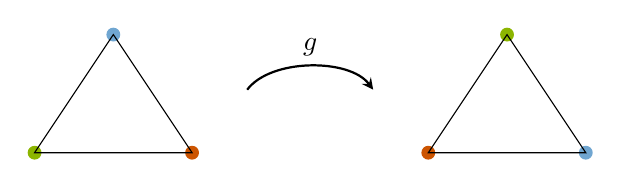
\begin{tikzpicture}[>=stealth]
        \tikzstyle{point}=[circle,fill,inner sep=0pt, minimum width=5pt, minimum height=5pt]
        \begin{scope}[shift={(-1,-.5)}]
            % Triangle vertices
            \node[iceberg] (e3)[point] at (1,1.5) {};
            \node[burntorange] (e1)[point] at (2,0) {};
            \node[applegreen] (e2)[point] at (0,0) {};

            % Barycenter
            \coordinate (bary) at (1,0.5) {}; 

            % Draw the triangle
            \draw (e1.center) -- (e2.center) -- (e3.center) -- cycle;
        \end{scope}
        % --- Curved arrow between them ---
    \draw[->, thick]
    (1.7,0.3) .. controls (2,0.7) and (3,0.7) .. (3.3,0.3)
    node[midway, above] {$g$};

        \begin{scope}[shift={(4,-.5)}]
            % Triangle vertices
            \node[applegreen] (e3)[point] at (1,1.5) {};
            \node[iceberg] (e1)[point] at (2,0) {};
            \node[burntorange] (e2)[point] at (0,0) {};

            % Barycenter
            \coordinate (bary) at (1,0.5) {}; 

            % Draw the triangle
            \draw (e1.center) -- (e2.center) -- (e3.center) -- cycle;
        \end{scope}
    \end{tikzpicture}
    \]
    Με άλλα λόγια, το $g$ δρα σαν την μετάθεση $\cycle{1,2,3}$ (γιατί;) και γι' αυτό έχει πίνακα 
    \[
    \begin{pmatrix}
        0 & 0 & 1 \\
        1 & 0 & 0 \\
        0 & 1 & 0
    \end{pmatrix}.
    \]
    Η δράση αυτή είναι πιστή (γιατί;) και γι' αυτό η $\rmC_3$ είναι ισόμορφη με την ακόλουθη υποομάδα της $\GL_3(\CC)$:
    \[
    \left\langle \begin{pmatrix}
        0 & 0 & 1 \\
        1 & 0 & 0 \\
        0 & 1 & 0
    \end{pmatrix} \right\rangle \ = \ 
    \left\{
    \begin{pmatrix}
        1 & 0 & 0 \\
        0 & 1 & 0 \\
        0 & 0 & 1
    \end{pmatrix}, \ 
    \begin{pmatrix}
        0 & 0 & 1 \\
        1 & 0 & 0 \\
        0 & 1 & 0
    \end{pmatrix}, \ 
    \begin{pmatrix}
        0 & 1 & 0 \\
        0 & 0 & 1 \\
        1 & 0 & 0
    \end{pmatrix}
    \right\}.
    \]

    Ποιός είναι ο πίνακας του στοιχείου $g$ στην κανονική αναπαράσταση της $\rmC_3$ ως προς την βάση $\{\textcolor{iceberg}{\epsilon}, \textcolor{burntorange}{g}, \textcolor{applegreen}{g^2}\}$; Τι παρατηρείτε;
\end{example}

\begin{example}{\rm($\rmD_6$-πρότυπα)}
    Η $\rmD_6$ δρα στο $[3]=\{\one, \two, \three\}$ με τους ακόλουθους τρεις τρόπους:
    \begin{itemize}
        \item[(1)] Σκεπτόμαστε τα στοιχεία του $[3]$ ως κορυφές ενός ισόπλευρου τριγώνου όπως πριν: 
        \[
    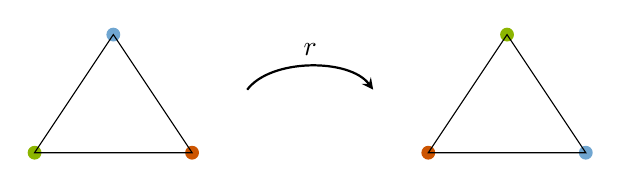
\begin{tikzpicture}[>=stealth]
        \tikzstyle{point}=[circle,fill,inner sep=0pt, minimum width=5pt, minimum height=5pt]
        \begin{scope}[shift={(-1,-.5)}]
            % Triangle vertices
            \node[iceberg] (e3)[point] at (1,1.5) {};
            \node[burntorange] (e1)[point] at (2,0) {};
            \node[applegreen] (e2)[point] at (0,0) {};

            % Barycenter
            \coordinate (bary) at (1,0.5) {}; 

            % Draw the triangle
            \draw (e1.center) -- (e2.center) -- (e3.center) -- cycle;
        \end{scope}
        % --- Curved arrow between them ---
    \draw[->, thick]
    (1.7,0.3) .. controls (2,0.7) and (3,0.7) .. (3.3,0.3)
    node[midway, above] {$r$};

        \begin{scope}[shift={(4,-.5)}]
            % Triangle vertices
            \node[applegreen] (e3)[point] at (1,1.5) {};
            \node[iceberg] (e1)[point] at (2,0) {};
            \node[burntorange] (e2)[point] at (0,0) {};

            % Barycenter
            \coordinate (bary) at (1,0.5) {}; 

            % Draw the triangle
            \draw (e1.center) -- (e2.center) -- (e3.center) -- cycle;
        \end{scope}
    \end{tikzpicture}
    \]
        με πίνακα 
        \[
    \begin{pmatrix}
        0 & 0 & 1 \\
        1 & 0 & 0 \\
        0 & 1 & 0
    \end{pmatrix}
    \]
    και 
    \[
    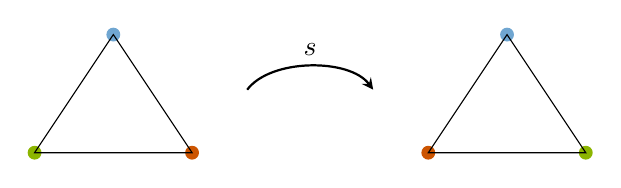
\begin{tikzpicture}[>=stealth]
        \tikzstyle{point}=[circle,fill,inner sep=0pt, minimum width=5pt, minimum height=5pt]
        \begin{scope}[shift={(-1,-.5)}]
            % Triangle vertices
            \node[iceberg] (e3)[point] at (1,1.5) {};
            \node[burntorange] (e1)[point] at (2,0) {};
            \node[applegreen] (e2)[point] at (0,0) {};

            % Barycenter
            \coordinate (bary) at (1,0.5) {}; 

            % Draw the triangle
            \draw (e1.center) -- (e2.center) -- (e3.center) -- cycle;
        \end{scope}
        % --- Curved arrow between them ---
    \draw[->, thick]
    (1.7,0.3) .. controls (2,0.7) and (3,0.7) .. (3.3,0.3)
    node[midway, above] {$s$};

        \begin{scope}[shift={(4,-.5)}]
            % Triangle vertices
            \node[iceberg] (e3)[point] at (1,1.5) {};
            \node[applegreen] (e1)[point] at (2,0) {};
            \node[burntorange] (e2)[point] at (0,0) {};
            
            % Barycenter
            \coordinate (bary) at (1,0.5) {}; 

            % Draw the triangle
            \draw (e1.center) -- (e2.center) -- (e3.center) -- cycle;
        \end{scope}
    \end{tikzpicture}
    \]
    με πίνακα 
     \[
    \begin{pmatrix}
        1 & 0 & 0 \\
        0 & 0 & 1 \\
        0 & 1 & 0
    \end{pmatrix}.
    \]
    \item[(2)] Σκεπτόμαστε τα στοιχεία του $[3]$ ως πλευρές ενός ισόπλευρου τριγώνου:
    \[
    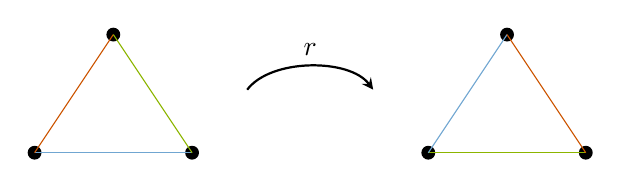
\begin{tikzpicture}[>=stealth]
        \tikzstyle{point}=[circle,fill,inner sep=0pt, minimum width=5pt, minimum height=5pt]
        \begin{scope}[shift={(-1,-.5)}]
            % Triangle vertices
            \node (e3)[point] at (1,1.5) {};
            \node (e1)[point] at (2,0) {};
            \node (e2)[point] at (0,0) {};

            % Barycenter
            \coordinate (bary) at (1,0.5) {}; 

            % Draw the triangle
            \draw[iceberg] (e1.center) -- (e2.center);
            \draw[burntorange] (e2.center) -- (e3.center);
            \draw[applegreen] (e3.center) -- (e1.center);
        \end{scope}
        % --- Curved arrow between them ---
    \draw[->, thick]
    (1.7,0.3) .. controls (2,0.7) and (3,0.7) .. (3.3,0.3)
    node[midway, above] {$r$};

        \begin{scope}[shift={(4,-.5)}]
            % Triangle vertices
            \node (e3)[point] at (1,1.5) {};
            \node (e1)[point] at (2,0) {};
            \node (e2)[point] at (0,0) {};
            
            % Barycenter
            \coordinate (bary) at (1,0.5) {}; 

            % Draw the triangle
            \draw[applegreen] (e1.center) -- (e2.center);
            \draw[iceberg] (e2.center) -- (e3.center);
            \draw[burntorange] (e3.center) -- (e1.center);
        \end{scope}
    \end{tikzpicture}
    \]
    και
    \[
    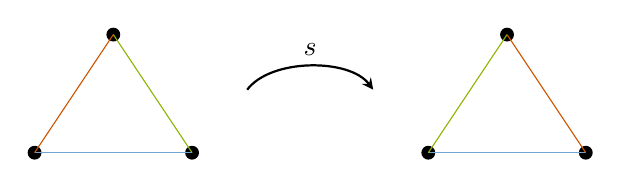
\begin{tikzpicture}[>=stealth]
        \tikzstyle{point}=[circle,fill,inner sep=0pt, minimum width=5pt, minimum height=5pt]
        \begin{scope}[shift={(-1,-.5)}]
            % Triangle vertices
            \node (e3)[point] at (1,1.5) {};
            \node (e1)[point] at (2,0) {};
            \node (e2)[point] at (0,0) {};

            % Barycenter
            \coordinate (bary) at (1,0.5) {}; 

            % Draw the triangle
            \draw[iceberg] (e1.center) -- (e2.center);
            \draw[burntorange] (e2.center) -- (e3.center);
            \draw[applegreen] (e3.center) -- (e1.center);
        \end{scope}
        % --- Curved arrow between them ---
    \draw[->, thick]
    (1.7,0.3) .. controls (2,0.7) and (3,0.7) .. (3.3,0.3)
    node[midway, above] {$s$};

        \begin{scope}[shift={(4,-.5)}]
            % Triangle vertices
            \node (e3)[point] at (1,1.5) {};
            \node (e1)[point] at (2,0) {};
            \node (e2)[point] at (0,0) {};
            
            % Barycenter
            \coordinate (bary) at (1,0.5) {}; 

            % Draw the triangle
            \draw[iceberg] (e1.center) -- (e2.center);
            \draw[applegreen] (e2.center) -- (e3.center);
            \draw[burntorange] (e3.center) -- (e1.center);
        \end{scope}
    \end{tikzpicture}
    \]
    Ποιοί είναι οι αντίστοιχοι πίνακες; Τι παρατηρείτε;
    \item[(3)] Σκεπτόμαστε τα στοιχεία του $[3]$ ως τις διαγώνιους ενός ισόπλευρου τριγώνου:
    \[
    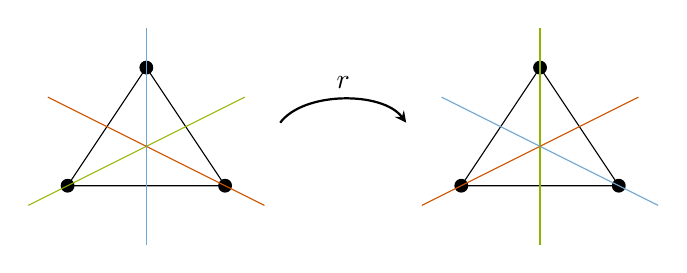
\begin{tikzpicture}[>=stealth]
        \tikzstyle{point}=[circle,fill,inner sep=0pt, minimum width=5pt, minimum height=5pt]
        \begin{scope}[shift={(-1,-.5)}]
            % Triangle vertices
            \node (e3)[point] at (1,1.5) {};
            \node (e1)[point] at (2,0) {};
            \node (e2)[point] at (0,0) {};

            % Barycenter
            \coordinate (bary) at (1,0.5) {}; 

            % Draw the triangle
        \draw (e1.center) -- (e2.center) -- (e3.center) -- cycle;

        % Compute extended axis endpoints
        \coordinate (e1_ext) at ($(bary) !1.5! (e1)$);
        \coordinate (e2_ext) at ($(bary) !1.5! (e2)$);
        \coordinate (e3_ext) at ($(bary) !1.5! (e3)$);

        % Draw coordinate axes
        \draw[iceberg] (bary.center) -- (e3_ext);
        \draw[burntorange] (bary.center) -- (e1_ext);
        \draw[applegreen] (bary.center) -- (e2_ext);

        % Make the e2 axis red and extend it beyond the midpoint of e1-e3
        \coordinate (mid_e1_e2) at ($(e1)!0.5!(e2)$); % Midpoint of e1 and e2
        \coordinate (mid_e1_e3) at ($(e1)!0.5!(e3)$); % Midpoint of e1 and e3
        \coordinate (mid_e2_e3) at ($(e2)!0.5!(e3)$); % Midpoint of e2 and e3
        \coordinate (e1_extended) at ($(e1)!1.5!(mid_e2_e3)$); % Extend e1 axis beyond midpoint
        \coordinate (e2_extended) at ($(e2)!1.5!(mid_e1_e3)$); % Extend e2 axis beyond midpoint
        \coordinate (e3_extended) at ($(e3)!1.5!(mid_e1_e2)$); % Extend e3 axis beyond midpoint
        \draw[iceberg] (bary.center) -- (e3_extended); % Red e3 axis extended
        \draw[applegreen] (bary.center) -- (e2_extended); % Red e2 axis extended
        \draw[burntorange] (bary.center) -- (e1_extended); % Red e1 axis extended
        \end{scope}
        % --- Curved arrow between them ---
    \draw[->, thick]
    (1.7,0.3) .. controls (2,0.7) and (3,0.7) .. (3.3,0.3)
    node[midway, above] {$r$};

        \begin{scope}[shift={(4,-.5)}]
            % Triangle vertices
            \node (e3)[point] at (1,1.5) {};
            \node (e1)[point] at (2,0) {};
            \node (e2)[point] at (0,0) {};
            
            % Barycenter
            \coordinate (bary) at (1,0.5) {}; 

            % Draw the triangle
        \draw (e1.center) -- (e2.center) -- (e3.center) -- cycle;

        % Compute extended axis endpoints
        \coordinate (e1_ext) at ($(bary) !1.5! (e1)$);
        \coordinate (e2_ext) at ($(bary) !1.5! (e2)$);
        \coordinate (e3_ext) at ($(bary) !1.5! (e3)$);

        % Draw coordinate axes
        \draw[iceberg] (bary.center) -- (e1_ext);
        \draw[burntorange] (bary.center) -- (e2_ext);
        \draw[applegreen] (bary.center) -- (e3_ext);

        % Make the e2 axis red and extend it beyond the midpoint of e1-e3
        \coordinate (mid_e1_e2) at ($(e1)!0.5!(e2)$); % Midpoint of e1 and e2
        \coordinate (mid_e1_e3) at ($(e1)!0.5!(e3)$); % Midpoint of e1 and e3
        \coordinate (mid_e2_e3) at ($(e2)!0.5!(e3)$); % Midpoint of e2 and e3
        \coordinate (e1_extended) at ($(e1)!1.5!(mid_e2_e3)$); % Extend e1 axis beyond midpoint
        \coordinate (e2_extended) at ($(e2)!1.5!(mid_e1_e3)$); % Extend e2 axis beyond midpoint
        \coordinate (e3_extended) at ($(e3)!1.5!(mid_e1_e2)$); % Extend e3 axis beyond midpoint
        \draw[applegreen] (bary.center) -- (e3_extended); % Red e3 axis extended
        \draw[burntorange] (bary.center) -- (e2_extended); % Red e2 axis extended
        \draw[iceberg] (bary.center) -- (e1_extended); % Red e1 axis extended
        \end{scope}
    \end{tikzpicture}
    \]
    και
    \[
    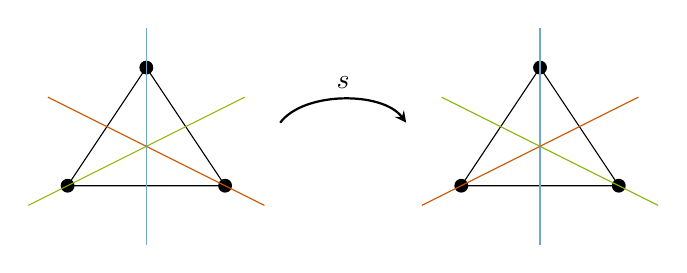
\begin{tikzpicture}[>=stealth]
        \tikzstyle{point}=[circle,fill,inner sep=0pt, minimum width=5pt, minimum height=5pt]
        \begin{scope}[shift={(-1,-.5)}]
            % Triangle vertices
            \node (e3)[point] at (1,1.5) {};
            \node (e1)[point] at (2,0) {};
            \node (e2)[point] at (0,0) {};

            % Barycenter
            \coordinate (bary) at (1,0.5) {}; 

            % Draw the triangle
        \draw (e1.center) -- (e2.center) -- (e3.center) -- cycle;

        % Compute extended axis endpoints
        \coordinate (e1_ext) at ($(bary) !1.5! (e1)$);
        \coordinate (e2_ext) at ($(bary) !1.5! (e2)$);
        \coordinate (e3_ext) at ($(bary) !1.5! (e3)$);

        % Draw coordinate axes
        \draw[iceberg] (bary.center) -- (e3_ext);
        \draw[burntorange] (bary.center) -- (e1_ext);
        \draw[applegreen] (bary.center) -- (e2_ext);

        % Make the e2 axis red and extend it beyond the midpoint of e1-e3
        \coordinate (mid_e1_e2) at ($(e1)!0.5!(e2)$); % Midpoint of e1 and e2
        \coordinate (mid_e1_e3) at ($(e1)!0.5!(e3)$); % Midpoint of e1 and e3
        \coordinate (mid_e2_e3) at ($(e2)!0.5!(e3)$); % Midpoint of e2 and e3
        \coordinate (e1_extended) at ($(e1)!1.5!(mid_e2_e3)$); % Extend e1 axis beyond midpoint
        \coordinate (e2_extended) at ($(e2)!1.5!(mid_e1_e3)$); % Extend e2 axis beyond midpoint
        \coordinate (e3_extended) at ($(e3)!1.5!(mid_e1_e2)$); % Extend e3 axis beyond midpoint
        \draw[iceberg] (bary.center) -- (e3_extended); % Red e3 axis extended
        \draw[applegreen] (bary.center) -- (e2_extended); % Red e2 axis extended
        \draw[burntorange] (bary.center) -- (e1_extended); % Red e1 axis extended
        \end{scope}
        % --- Curved arrow between them ---
    \draw[->, thick]
    (1.7,0.3) .. controls (2,0.7) and (3,0.7) .. (3.3,0.3)
    node[midway, above] {$s$};

        \begin{scope}[shift={(4,-.5)}]
            % Triangle vertices
            \node (e3)[point] at (1,1.5) {};
            \node (e1)[point] at (2,0) {};
            \node (e2)[point] at (0,0) {};
            
            % Barycenter
            \coordinate (bary) at (1,0.5) {}; 

            % Draw the triangle
        \draw (e1.center) -- (e2.center) -- (e3.center) -- cycle;

        % Compute extended axis endpoints
        \coordinate (e1_ext) at ($(bary) !1.5! (e1)$);
        \coordinate (e2_ext) at ($(bary) !1.5! (e2)$);
        \coordinate (e3_ext) at ($(bary) !1.5! (e3)$);

        % Draw coordinate axes
        \draw[iceberg] (bary.center) -- (e3_ext);
        \draw[applegreen] (bary.center) -- (e1_ext);
        \draw[burntorange] (bary.center) -- (e2_ext);

        % Make the e2 axis red and extend it beyond the midpoint of e1-e3
        \coordinate (mid_e1_e2) at ($(e1)!0.5!(e2)$); % Midpoint of e1 and e2
        \coordinate (mid_e1_e3) at ($(e1)!0.5!(e3)$); % Midpoint of e1 and e3
        \coordinate (mid_e2_e3) at ($(e2)!0.5!(e3)$); % Midpoint of e2 and e3
        \coordinate (e1_extended) at ($(e1)!1.5!(mid_e2_e3)$); % Extend e1 axis beyond midpoint
        \coordinate (e2_extended) at ($(e2)!1.5!(mid_e1_e3)$); % Extend e2 axis beyond midpoint
        \coordinate (e3_extended) at ($(e3)!1.5!(mid_e1_e2)$); % Extend e3 axis beyond midpoint
        \draw[iceberg] (bary.center) -- (e3_extended); % Red e3 axis extended
        \draw[burntorange] (bary.center) -- (e2_extended); % Red e2 axis extended
        \draw[applegreen] (bary.center) -- (e1_extended); % Red e1 axis extended
        \end{scope}
    \end{tikzpicture}
    \]
    Ποιοί είναι οι αντίστοιχοι πίνακες; Τι παρατηρείτε;
    \end{itemize}
\end{example}

\begin{example}{\rm($\rmV_4$-πρότυπα)}
    Έστω $\rmV_4$ η \defn{4-ομάδα του Klein} με παράσταση
    \[
    \rmV_4 \coloneqq 
    \langle a, b \ \vert \ a^2 = b^2 = (ab)^2 = \epsilon \rangle  \cong \rmC_2 \times \rmC_2.
    \]
    Η $\rmV_4$ είναι η μικρότερη μη-κυκλική ομάδα και προκύπτει ως ομάδα συμμετρίας του ρόμβου
    \[
    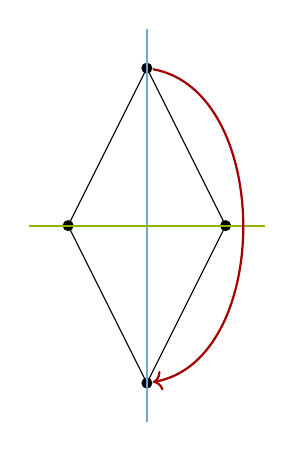
\begin{tikzpicture}
        % Define the point style
        \tikzstyle{point}=[circle,fill,inner sep=0pt, minimum width=4pt, minimum height=4pt]

        % Rhombus vertices
        \node (A)[point] at (0,2) {};
        \node (B)[point] at (1,0) {};
        \node (C)[point] at (0,-2) {};
        \node (D)[point] at (-1,0) {};

        % Barycenter (center of symmetry)
        \coordinate (center) at (0,0);

        % Draw the rhombus
        \draw (A.center) -- (B.center) -- (C.center) -- (D.center) -- cycle;

        % Lines of symmetry
        \draw[thick, iceberg] (0,-2.5) -- (0,2.5);  % Vertical axis
        \draw[thick, applegreen] (-1.5,0) -- (1.5,0);     % Horizontal axis

        % Curved arrow from A to C around the right side
        \draw[->, thick, bend left=80, darkcandyapplered] (A) to (C);
    \end{tikzpicture}
    \]
    όπου 
    \begin{itemize}
        \item $a$ είναι η ανάκλαση ως προς τον οριζόντιο άξονα, και
        \item $b$ είναι η ανάκλαση ως προς τον κάθετο άξονα.
    \end{itemize}
    Συνεπώς, $ab$ είναι η στροφή κατά τη φορά του ρολογιού κατά $\pi$ (γιατί;). Πως επαληθεύονται σχηματικά οι σχέσεις;

    Όπως και στην περίπτωση των $\rmD_6$-προτύπων η $\rmV_4$ δρα στο σύνολο $[4]$, το οποίο μπορούμε να σκεφτούμε ως τις κορυφές, τις πλευρές και τις διαγώνιους του ρόμβου. Ποιοί είναι οι αντίστοιχοι πίνακες; Ποιές είναι αντίστοιχες αναπαραστάσεις μεταθέσεων; Προκύπτουν ισόμορφα πρότυπα ή μη;
\end{example}

\begin{example}{\rm($\rmD_8$-πρότυπα)}
    Όμοια με τα προηγούμενα παραδείγματα, η $\rmD_8$ δρα στο $[4] = \{\one, \two, \three, \four\}$ το οποίο μπορούμε να σκεφτούμε ως τις κορυφές, τις πλευρές και τις διαγώνιους του ρόμβου. Στην περίπτωση αυτή όμως, οι επαγώμενες αναπαραστάσεις μεταθέσεων \emph{δεν} είναι ισόμορφες. Για παράδειγμα, η δράση της απεικονιζόμενης ανάκλασης στις κορυφές
    \[
    \begin{tikzpicture}
        \tikzstyle{point}=[circle,fill,inner sep=0pt, minimum width=4pt, minimum height=4pt]
        \begin{scope}[shift={(0,0)}]
        % Square vertices
        \coordinate (v1) at (1,1);    % upper right
        \coordinate (v2) at (1,-1);   % lower right
        \coordinate (v3) at (-1,-1);  % lower left
        \coordinate (v4) at (-1,1);   % upper lef
        % Draw vertices as filled points and label
        \node[point,iceberg] at (v1) {};
        \node[point,burntorange] at (v2) {};
        \node[point,applegreen] at (v3) {};
        \node[point,canaryyellow] at (v4) {};
        % center (barycenter)
        \coordinate (O) at (0,0);
        % midpoints of edges (medians direction)
        \coordinate (m12) at ($(v1)!0.5!(v2)$); % (1,0)
        \coordinate (m23) at ($(v2)!0.5!(v3)$); % (0,-1)
        \coordinate (m34) at ($(v3)!0.5!(v4)$); % (-1,0)
        \coordinate (m41) at ($(v4)!0.5!(v1)$); % (0,1)
        % Draw square
        \draw (v1) -- (v2) -- (v3) -- (v4) -- cycle;
        % Median horizontal (through midpoints m12 and m34)
        \draw[dashed]
            ($(O)!1.4!(m12)$) -- ($(O)!-1.4!(m12)$);
        \end{scope}
        \coordinate[label={$\mapstoto$}] (x) at (2.2,-0.25);
        \begin{scope}[shift={(4.5,0)}]
        % Square vertices
        \coordinate (v1) at (1,1);    % upper right
        \coordinate (v2) at (1,-1);   % lower right
        \coordinate (v3) at (-1,-1);  % lower left
        \coordinate (v4) at (-1,1);   % upper lef
        % Draw vertices as filled points and label
        \node[point,burntorange] at (v1) {};
        \node[point,iceberg] at (v2) {};
        \node[point,canaryyellow] at (v3) {};
        \node[point,applegreen] at (v4) {};
        % center (barycenter)
        \coordinate (O) at (0,0);
        % midpoints of edges (medians direction)
        \coordinate (m12) at ($(v1)!0.5!(v2)$); % (1,0)
        \coordinate (m23) at ($(v2)!0.5!(v3)$); % (0,-1)
        \coordinate (m34) at ($(v3)!0.5!(v4)$); % (-1,0)
        \coordinate (m41) at ($(v4)!0.5!(v1)$); % (0,1)
        % Draw square
        \draw (v1) -- (v2) -- (v3) -- (v4) -- cycle;
        % Median horizontal (through midpoints m12 and m34)
        \draw[dashed]
            ($(O)!1.4!(m12)$) -- ($(O)!-1.4!(m12)$);
        \end{scope}
    \end{tikzpicture}
    \]
    δεν έχει σταθερά σημεία, ενώ η αντίστοιχη στις ακμές
    \[
    \begin{tikzpicture}
        \tikzstyle{point}=[circle,fill,inner sep=0pt, minimum width=4pt, minimum height=4pt]
        \begin{scope}[shift={(0,0)}]
        % Draw vertices as filled points and label
        \node (v1)[point] at (1,1) {};
        \node (v2)[point] at (1,-1) {};
        \node (v3)[point] at (-1,-1) {};
        \node (v4)[point] at (-1,1) {};
        % center (barycenter)
        \coordinate (O) at (0,0);
        % midpoints of edges (medians direction)
        \coordinate (m12) at ($(v1)!0.5!(v2)$); % (1,0)
        \coordinate (m23) at ($(v2)!0.5!(v3)$); % (0,-1)
        \coordinate (m34) at ($(v3)!0.5!(v4)$); % (-1,0)
        \coordinate (m41) at ($(v4)!0.5!(v1)$); % (0,1)
        % Draw square
        \draw[iceberg] (v1.center) -- (v2.center);
        \draw[burntorange] (v2.center) -- (v3.center);
        \draw[applegreen] (v3.center) -- (v4.center);
        \draw[canaryyellow] (v4.center) -- (v1.center);
        % Median horizontal (through midpoints m12 and m34)
        \draw[dashed]
            ($(O)!1.4!(m12)$) -- ($(O)!-1.4!(m12)$);
        \end{scope}
        \coordinate[label={$\mapstoto$}] (x) at (2.2,-0.25);
        \begin{scope}[shift={(4.5,0)}]
        % Draw vertices as filled points and label
        \node (v1)[point] at (1,1) {};
        \node (v2)[point] at (1,-1) {};
        \node (v3)[point] at (-1,-1) {};
        \node (v4)[point] at (-1,1) {};
        % center (barycenter)
        \coordinate (O) at (0,0);
        % midpoints of edges (medians direction)
        \coordinate (m12) at ($(v1)!0.5!(v2)$); % (1,0)
        \coordinate (m23) at ($(v2)!0.5!(v3)$); % (0,-1)
        \coordinate (m34) at ($(v3)!0.5!(v4)$); % (-1,0)
        \coordinate (m41) at ($(v4)!0.5!(v1)$); % (0,1)
        % Draw square
        \draw[iceberg] (v1.center) -- (v2.center);
        \draw[canaryyellow] (v2.center) -- (v3.center);
        \draw[applegreen] (v3.center) -- (v4.center);
        \draw[burntorange] (v4.center) -- (v1.center);
        % Median horizontal (through midpoints m12 and m34)
        \draw[dashed]
            ($(O)!1.4!(m12)$) -- ($(O)!-1.4!(m12)$);
        \end{scope}
    \end{tikzpicture}
    \]
    αφήνει σταθερά τα στοιχεία $\{\one, \three\}$. Έχει σημασία πως θα χρωματίσουμε τα στοιχεία του $[4]$;
    Ποιά είναι η δράση του $\rmD_8$ στις διαγώνιους τους τετραγώνου; Είναι πιστή; Τι παρατηρείτε;

    Η $\rmD_8$ έχει τέσσερις \emph{διαφορετικές} αναπαραστάσεις διάστασης 1, οι οποίες προκύπτουν από τις εξείς δράσεις στους γεννήτορες:
    \[
    \begin{aligned}
    r &\mapsto 1, \quad &s &\mapsto 1\\
    r &\mapsto 1, \quad &s &\mapsto -1\\
    r &\mapsto -1, \quad &s &\mapsto 1\\
    r &\mapsto -1, \quad &s &\mapsto -1
    \end{aligned}
    \]
    (γιατί;) Η $\rmD_6$, η οποία είναι ισόμορφη με την $\fS_3$, είδαμε ότι έχει δυο, την τετριμμένη και την αναπαράσταση προσήμου:
    \[
    \begin{aligned}
    r &\mapsto 1, \quad &s &\mapsto 1\\
    r &\mapsto 1, \quad &s &\mapsto -1\\
    \end{aligned}
    \]
    (γιατί;). Πως γενικεύεται αυτό για αυθαίρετο $n$;
\end{example}

\begin{combInterlude}
    Το σύνολο των διαγωνίων (ως ευθείες) του τριγώνου και του τετραγώνου στο επίπεδο είναι παράδειγμα παρατάγματος υπερεπιπέδου. Γενικότερα, \defn{παράταγμα υπερεπιπέδου} (hyperplane arrangement) ονομάζεται ένα σύνολο \emph{υπερεπιπέδων} στον $\RR^n$, δηλαδή υπόχωρων της μορφής 
    \[
    \{v \in \RR^n : v\cdot\alpha = 0\},
    \]
    όπου $\alpha$ είναι ένα μη-μηδενικό διάνυσμα και $\cdot$ είναι το σύνηθες εσωτερικό γινόμενο στον $\RR^n$.

    Δοθέντος ενός παρατάγματος επιπέδου $\aA$, έχει νόημα να κοιτάξουμε το συμπλήρωμα $\RR^n\sm\aA$ και να αναρωτηθούμε ποιό είναι το πλήθος των συννεκτικών συνιστοσών του. Στην περίπτωση του τριγώνου έχουμε 6 συνεκτικές συνιστώσες, όσα και τα στοιχεία της $\fS_3$ (της ομάδας συμμετρίας του τριγώνου αυτού)! 

    Τα παρατάγματα υπερεπιπέδων αποτελούν βασικό αντικείμενο μελέτης της απαριθμητικής και γεωμετρικής συνδυαστικής. 
\end{combInterlude}
\end{document}